\section{Hello World!}
\begin{frame}{Reto}
    \Huge\centering\textbf{ROM HACKING TIME!}
\end{frame}

\subsection{Conceptos}
\begin{frame}[fragile]{Números hexadecimales}
    \begin{uncoverenv}<2->Decimal: 0 1 2 3 4 5 6 7 8 9
    \begin{lstlisting}
    0 1 2 3 4 5 6 7 8 9 10 11 12 13 ...\end{lstlisting}\end{uncoverenv}

    \begin{uncoverenv}<3->Binario: 0 1
    \begin{lstlisting}
    0 1 10 11 100 101 110 111 1000 ...
    0 1  2  3   4   5   6   7    8\end{lstlisting}\end{uncoverenv}

    \begin{uncoverenv}<4->Octal: 0 1 2 3 4 5 6 7
    \begin{lstlisting}
    0 1 2 3 4 5 6 7 10 11 12 13 14 ...
    0 1 2 3 4 5 6 7  8  9 10 11 12\end{lstlisting}\end{uncoverenv}

    \begin{uncoverenv}<5->Hexadecimal: 0 1 2 3 4 5 6 7 8 9 A B C D E F
    \begin{lstlisting}
    0 1 2 3 4 5 6 7 8 9  A  B  C  D  E  F 10 11 12 ...
    0 1 2 3 4 5 6 7 8 9 10 11 12 13 14 15 16 17 18\end{lstlisting}\end{uncoverenv}
\end{frame}

\begin{frame}[fragile]{Números hexadecimales}
    \begin{wideitemize}
        \item<1-> Prefijo \texttt{0x} o sufijo \texttt{h} \\
        \texttt{0xA, FBh, 0xCA, FEh}

        \item<2-> Fácil representación de enteros:
    \end{wideitemize}
    \visible<2->{\footnotesize\ctable[]{cccccl}{}{                          \FL
        \# & Rango & Ejemplo & Bytes & Bits & Otros nombres                 \ML
        1 & \texttt{[0, 15]} & \texttt{0xC} & \textonehalf & 4 &            \NN
        2 & \texttt{[0, 255]} & \texttt{0xC0} & 1 & 8 & byte                \NN
        4 & \texttt{[0, 65,535]} & \texttt{0x0200} & 2 & 16 & ushort, WORD  \NN
        8 & \texttt{[0, 4,294,967,295]} & \texttt{0xB7000000} & 4 & 32 & uint, DWORD \LL
    }}
\end{frame}

\begin{frame}{Números hexadecimales}
    Operaciones a nivel de bits:
    \small
    \begin{itemize}
        \item<3-> Filtrar/Máscaras:\\\texttt{0xAFC2 AND 0xF800 = 0xA800}
        \item<4-> Formar valores:\\\texttt{0xB7000000 OR 0xCADB00 = 0xB70ADB00}
        \item<5-> Cifrar:\\\texttt{0xCAFE XOR 0xAAAA = 0x6054, NOT 0xBEBE = 0x3501}
        \item<6-> Desplazamientos:\\\texttt{0xC2 << 4 = 0xC20, 0xA800 >> 8 = 0xA8}
    \end{itemize}
    \visible<2->{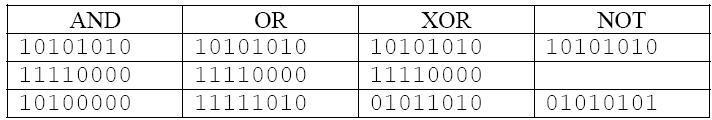
\includegraphics[width=\textwidth]{imgs/bitop.png}}
\end{frame}


\begin{frame}{Endianness}
    \begin{block}{}
        Orden en el que se guardan los bytes que forman valores mayores a 8 bits (ushort, uint, ulong, \ldots). MSB \textrightarrow LSB.
    \end{block}
    \centering{}\uncover<2->{Big Endian:}
    \visible<2->{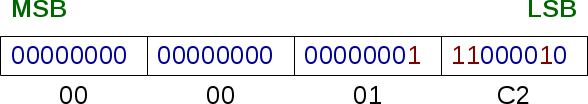
\includegraphics[width=0.9\textwidth]{imgs/big_endian.png}}
    \vfill
    \uncover<3->{Little Endian (más común):}
    \visible<3->{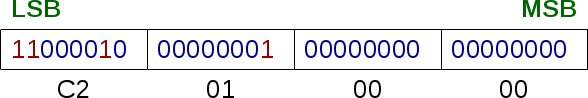
\includegraphics[width=0.9\textwidth]{imgs/little_endian.png}}
\end{frame}

\subsection{Investigando un juego}
\begin{frame}{Especificación de juegos de NDS}
    \begin{block}{GBATEK}
        \centering
         Gameboy Advance / Nintendo DS / DSi - Technical Info \\
         Trabajo de Martin Korth en el desarrollo de no\$gba.
        \url{http://problemkaputt.de/gbatek.htm}
    \end{block}
    \vfill
    \small
    \begin{columns}
    \begin{column}{0.3\textwidth}
        \uncover<2->{Cabecera\\}
        \uncover<3->{Binario ARM9\\}
        \uncover<3->{Overlays ARM9}
    \end{column}
    \begin{column}{0.3\textwidth}
        \uncover<3->{Binario ARM7\\}
        \uncover<3->{Overlays ARM7\\}
        \uncover<4->{File Name Table}
    \end{column}
    \begin{column}{0.3\textwidth}
        \uncover<4->{File Allocation Table\\}
        \uncover<5->{Banner\\}
        \uncover<6->{Archivos}
    \end{column}
    \end{columns}
\end{frame}

\begin{frame}{Tinke}
    % Abrir tinke, acciones típicas y significado de iconos
    \only<1>{\includefigure{Tinke}{imgs/tinke.png}{1}}
    \only<2>{\includefigure{Interfaz}{imgs/tinke_preview.png}{1}}
\end{frame}

\begin{frame}{Tipos de ficheros}
    \begin{columns}
    \begin{column}{0.5\textwidth}
        \begin{itemize}
            \item Paleta 
\includegraphics{imgs/palette.png}
            \item Tiles 
\includegraphics{imgs/picture.png}
            \item Map 
\includegraphics{imgs/picture_link.png}
            \item Sprites 
\includegraphics{imgs/pictures.png}
            \item Animaciones 
\includegraphics{imgs/picture_go.png}
            \item Modelos 3D 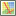
\includegraphics{imgs/map.png}
            \item Texturas 
\includegraphics{imgs/image.png}
            \item Imagen completa 
\includegraphics{imgs/photo.png}
        \end{itemize}
    \end{column}
    \hfill
    \begin{column}{0.5\textwidth}
        \begin{itemize}
            \item Texto 
\includegraphics{imgs/page_white_text.png}
            \item Tipografía 
\includegraphics{imgs/font.png}
            \item Scripts 
\includegraphics{imgs/script.png}
            \item Archivo comprimido 
\includegraphics{imgs/compress.png}
            \item Paquete 
\includegraphics{imgs/package.png}
            \item Música 
\includegraphics{imgs/music.png}
            \item Vídeo 
\includegraphics{imgs/film.png}
        \end{itemize}
    \end{column}
    \end{columns}
\end{frame}

\subsection{Editar juegos}
\begin{frame}{Modificando textos}
    \begin{columns}
    \begin{column}{0.5\textwidth}
        \begin{enumerate}
            \item<1-> Localizar texto a modificar
            \item<2-> Abrir juego en Tinke
            \item<3-> Localizar textos
            \item<4-> Extraer archivo
            \item<5-> Modificar con editor
            \item<6-> Importar archivo
            \item<7-> Generar ROM
            \item<8-> Probar en DeSmuME
        \end{enumerate}
    \end{column}
    \hfill
    \begin{column}{0.5\textwidth}
        \centering
        \only<1>{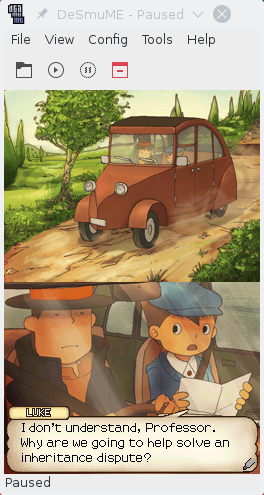
\includegraphics[width=0.7\textwidth]{imgs/mod1.png}}
        \only<2>{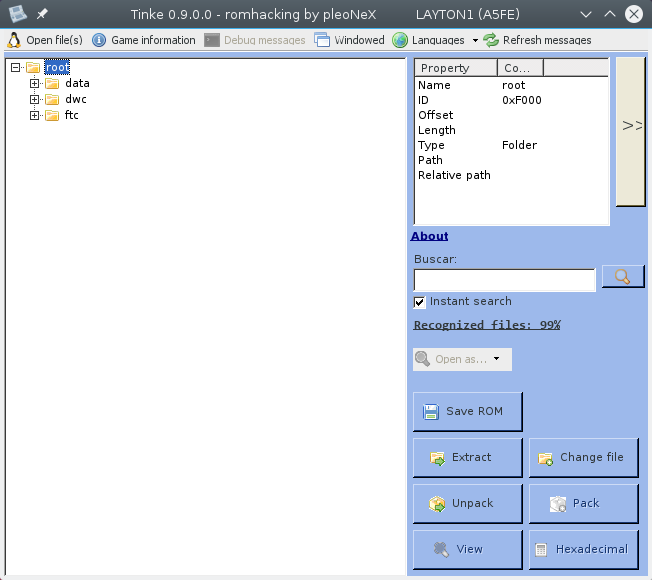
\includegraphics[width=\textwidth]{imgs/mod2.png}}
        \only<3>{\includegraphics[width=\textwidth]{imgs/mod3.png}}
        \only<4>{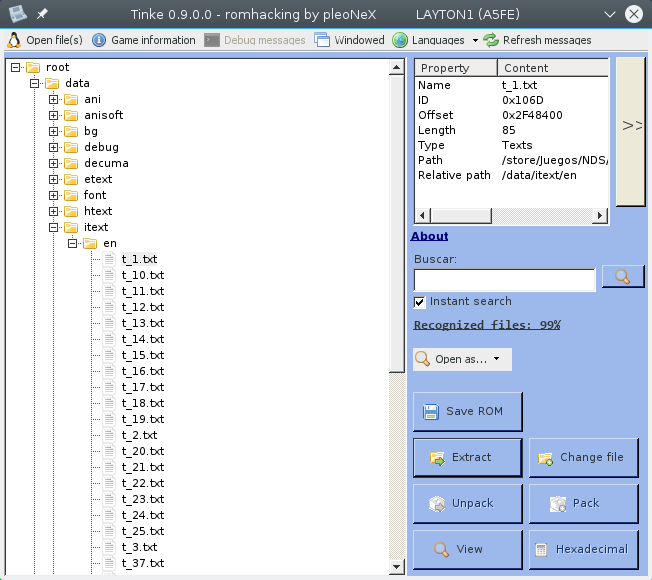
\includegraphics[width=\textwidth]{imgs/mod4.png}}
        \only<5>{\includegraphics[width=\textwidth]{imgs/mod5.png}}
        \only<6>{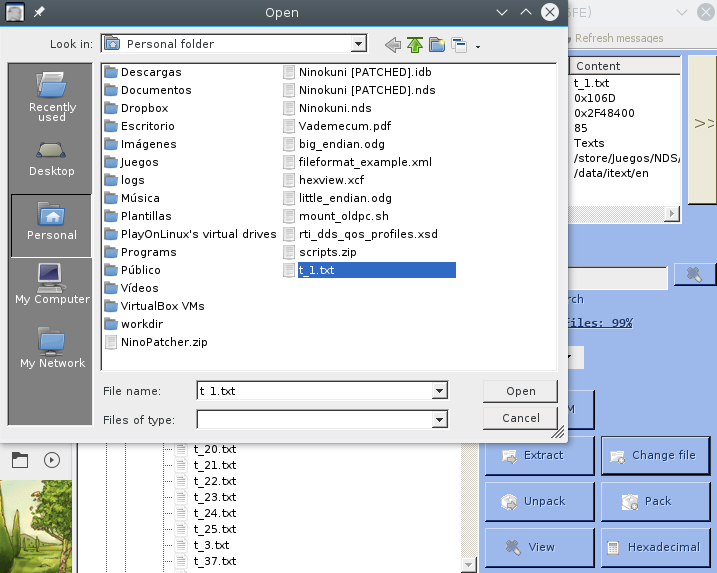
\includegraphics[width=\textwidth]{imgs/mod6.png}}
        \only<7>{\includegraphics[width=\textwidth]{imgs/mod7.png}}
        \only<8>{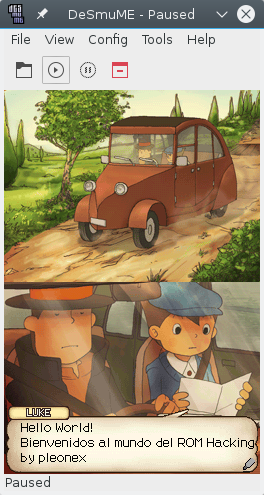
\includegraphics[width=0.7\textwidth]{imgs/mod8.png}}
        \only<9>{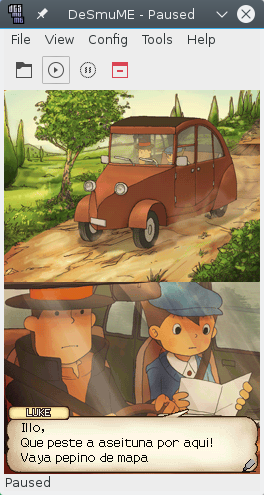
\includegraphics[width=0.7\textwidth]{imgs/pepino.png}}
    \end{column}
    \end{columns}
\end{frame}

\subsection{Distribuyamos los cambios}
\begin{frame}{Legalidad}
    \begin{block}{Ingeniería inversa en España}<+->
        En España es legal siempre y cuando se cuente con una copia del producto original.
    \end{block}
    \begin{block}{Ingeniería inversa en EEUU}<+->
        En EEUU la ley DMCA la prohíbe aunque hay juicios favorables de la Corte Suprema americana definiéndola como \textit{una parte esencial de la innovación}.
    \end{block}
    \begin{block}{ROM Hacking}<+->
        De los cientos de traducciones y mods disponibles solo ha habido unos pocos C\&D.
    \end{block}
\end{frame}

\begin{frame}{Parches}
    \begin{columns}
    \begin{column}{0.6\textwidth}
        \small
        \begin{wideitemize}
            \item<1-> Solo contienen las modificaciones
            \item<1-> \textbf{No subir el juego modificado}
            \item<2-> Tamaño pequeño (entre 1 y 20 MB)
            \item<3-> Formatos comunes: IPS y xDelta
        \end{wideitemize}
    \end{column}
    \begin{column}{0.4\textwidth}
        \includegraphics[width=\textwidth]{imgs/ninopatcher.png}
    \end{column}
    \end{columns}
\end{frame}

\begin{frame}{xDelta}
    \begin{columns}
    \begin{column}{0.7\textwidth}
        \footnotesize
        \begin{wideitemize}
            \item<1-> Windows: xdelta UI \\ \url{http://www.romhacking.net/utilities/598/}

            \item<2-> Mac OS X: Multipatch \\ \url{http://projects.sappharad.com/tools/multipatch.html}

            \item<3-> Linux: xdelta
            \begin{itemize}
                \footnotesize
                \item Parchear: \\ \texttt{xdelta -d -s ORIGINAL PARCHE}
                \item Crear parche: \\ \texttt{xdelta -9 -s ORIGINAL MODIFICADO PARCHE}
            \end{itemize}
        \end{wideitemize}
    \end{column}
    \begin{column}{0.3\textwidth}
        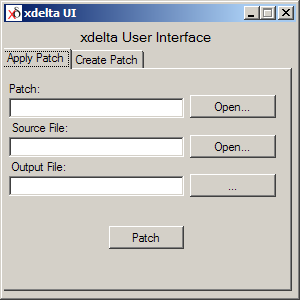
\includegraphics[width=\textwidth]{imgs/xdelta_windows.png}
        \vfill
        \visible<2->{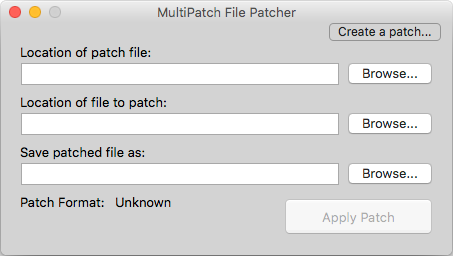
\includegraphics[width=\textwidth]{imgs/xdelta_mac.png}}
    \end{column}
    \end{columns}
\end{frame}
